\section{การลบบทบรรยายบนอนิเมะ}
\hspace{1cm} สำหรับการลบบทบรรยายอนิเมะ จะใช้วิดีโอ Anime Festival Asia Special Video - feat. Inori Aizawa ซึ่งผลิตโดย Collateral Damage Studios โดยจะตัดวิดีโอ 1 นาทีแรกสำหรับการทดลอง โดยวิดีโอดังกล่าวขนาด 1280 x 720 พิกเซล แต่เนื่องจากโดยปกติแล้ว อนิเมะมักมีบรรทัดเพียง 1 ถึง 2 บรรทัด จึงทำการแบ่งวิดีโอออกอีกเป็น 5 ส่วนได้ขนาดเป็น 1280 x 144 พิกเซลก่อนนำไปทดสอบในลำดับถัดไป
\hspace{1cm} และสำหรับบทบรรยายที่จะใช้ทดสอบนั้น เนื่องจากวิดีโอ Anime Festival Asia Special Video - feat. Inori Aizawa ไม่มีคำพูดใดๆ จึงใช้บทความ lorem ipsum เป็นบทบรรยาย โดยจะทำการแสดงบทบรรยาย 1 บรรทัด ความยาว 3 วินาที ทุก 2 วินาที นั่นคือในวิดีโอดังกล่าวจะมีบทบรรยายทั้งสิ้น 20 บรรทัด	
	
\begin{figure}[H]
    \centering
    \begin{subfigure}{0.8\linewidth}
        \centering
        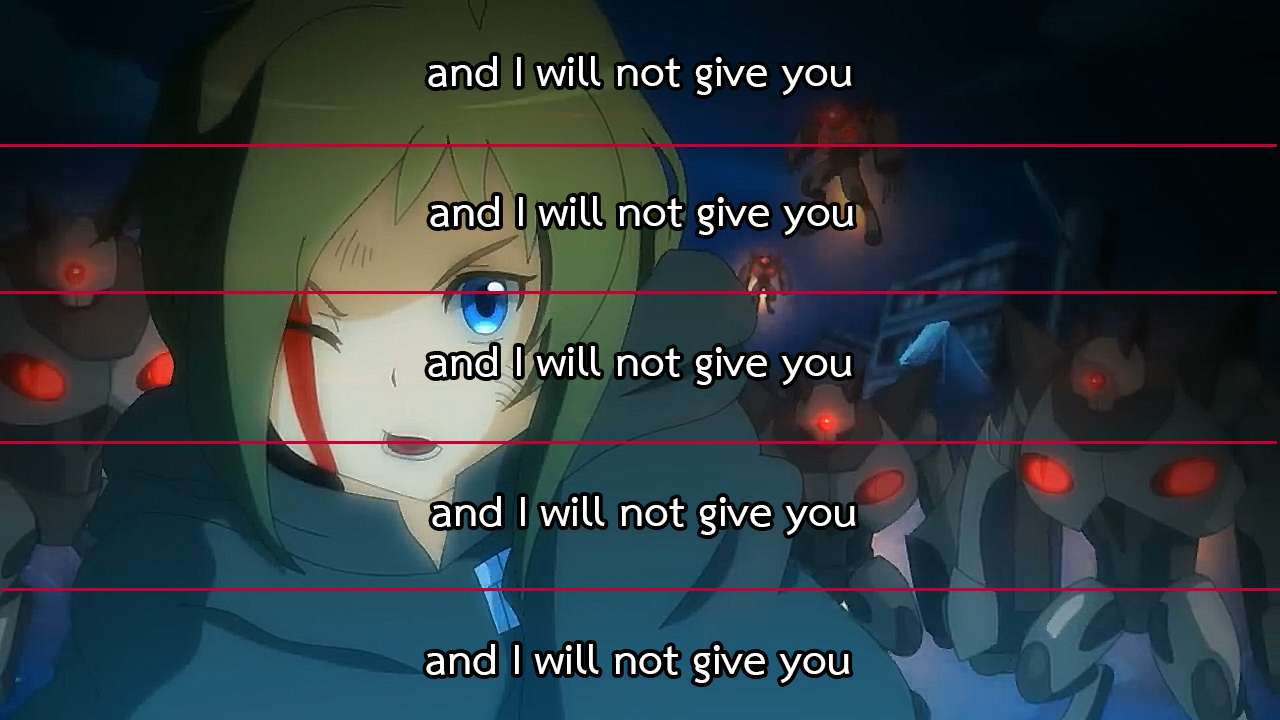
\includegraphics[width=0.8\linewidth]{image/inori-subbed-preview.png}
    \end{subfigure}
    \caption{การแบ่งไฟล์วิดีโอเป็น 5 ส่วนสำหรับใช้เป็น 5 ชุดทดสอบ}
\end{figure}

\subsection{การหาบทบรรยายบนอนิเมะ}	
    
\hspace{1cm} วิธีการหาบทบรรยายที่กล่าวไปข้างต้น จะทำการทดสอบกับบทความ lorem ipsum\footnote{Cicero, De finibus bonorum et malorum; เข้าถึงได้ทาง https://en.wikipedia.org/wiki/Lorem\_ipsum สืบค้นเมื่อวันที่ 23 ตุลาคม 2561} ที่ถูกแปลเป็นภาษาไทย ภาษาอังกฤษ และภาษาญี่ปุ่น โดยมีความสามารถในการหาโดเมนต่อเติมใบบทบรรยายภาษาต่างๆ ดังนี้

\begin{table}[H]
    \centering
    \footnotesize
    \begin{tabular}[ht]{|l|c|c|c|c|c|}
        \hline
        ภาษา  & วีดีโอ & จำนวนพิกเซลในโดเมน & จำนวนพิกเซลที่ตรวจพบ & จำนวนพิกเซลที่ผิดพลาด & ร้อยละการผิดพลาด \\
        \hline
        ไทย & 1 & 23,190,522  & 24,044,004 & 2,108,772 &9.09\\
             & 2 & 23,232,287 & 24,026,820 & 2,204,025 & 9.49\\
            & 3 & 23,189,082 & 24,300,589 & 2,081,340 & 8.98\\
            & 4 & 23,277,706 & 23,796,276  & 2,126,004 & 9.13\\
            & 5 & 23,221,502 & 24,247,935 & 2,185,864 & 9.41\\
        \hline
        อังกฤษ & 1 & 27,281,185 & 28,631,063 & 3,477,960  & 12.75\\
        & 2 & 27,269,671 & 28,513,248 & 3,514,859 & 12.89\\
        & 3 & 27,325,148 & 28,611,300 & 3,815,082 & 13.96\\
        & 4 & 27,191,136 & 28,527,105 & 3,854,121 & 14.17\\
        & 5 & 27,326,584 & 28,709,405 & 3,909,582 & 14.31\\
        \hline
        ญี่ปุ่น & 1 & 28,509,908 & 30,058,101 &  3,953,067 & 13.87\\
        & 2 & 28,534,363  & 30,023,923 & 3,565,609 & 12.50\\
        & 3 & 28,537,968 & 30,015,047 & 3,553,128 & 12.45\\
        & 4 & 28,579,778 & 30,065,985 & 3,961,319 & 13.86\\
        & 5 & 28,558,848 & 30,354,275 & 3,671,730 & 12.86\\
        \hline
    \end{tabular}
    \caption{ความคลาดเคลื่อนของการหาโดเมนต่อเติม ในบทบรรยายภาษาต่างๆ}
\end{table}
\begin{table}[H]
    \centering
        \footnotesize
    \begin{tabular}[ht]{|l|c|c|c|c|}
        \hline
        ภาษา  & จำนวนพิกเซลในโดเมน & จำนวนพิกเซลที่ตรวจพบ & จำนวนพิกเซลที่ผิดพลาด & ร้อยละการผิดพลาด \\
        \hline
        ไทย & 23,222,220 & 24,083,125 & 2,141,201 & 9.22 \\
        อังกฤษ & 27,278,745 & 28,598,424 & 3,714,321 & 13.62 \\
        ญี่ปุ่น & 28,544,173 & 30,103,466 & 3,740,971 & 13.11 \\
        \hline
    \end{tabular}
    \caption{ความคลาดเคลื่อนเฉลี่ยของการหาโดเมนต่อเติม ในบทบรรยายภาษาต่างๆ}
\end{table}	
	

\hspace{1cm} จากการทดลองทั้ง  3 ภาษาพบว่าวิธีการหาคำบรรยายนี้ มีร้อยละการผิดพลาดเฉลี่ยอยู่ที่ 11.98 ซึ่งการทดลองจากนี้ไปจะใช้วิธีการหาคำบรรยายนี้ในการหาโดเมนต่อเติมแบบอัตโนมัติ

\subsection{การลบคำบรรยายจากบทอนิเมะ}

\hspace{1cm} สำหรับอนิเมะนั้น แต่ละเฟรมจะเป็นรูปภาพ เราจึงสามารถประยุกต์ใช้วิธีการซ่อมแซมภาพจิตรกรรมไทย มาใช้ในการลบคำบรรยายได้ แต่ผู้วิจัยก็ได้สังเกตว่า สำหรับอนิเมะที่เป็นวิดีโอแล้ว ในขณะที่ประมวลผลวิดีโอ จะสามารถใช้ผลการต่อเติมภาพจากภาพที่แล้ว มาใช้เป็นคำตอบเริ่มต้นจึงได้ว่าขึ้นตอนการลบบทบรรยายออกจากวิดีโอ ซึ่งผลลัพธ์เปรียบเทียบระหว่างแบบใช้วิธี ยืมเฟรม ใช้วิธีข้ามเฟรม และวิธีข้ามและยืมเฟรม ได้ผลดังตาราง

\begin{table}[H]
    \small
    \centering
    \begin{tabular}[ht]{|l|c|c|c|c|c|}
        \hline
        วิธีการ  & วิดีโอ &เวลาประมวล  (วินาที) & PSNR (dB) & SSIM \\
        \hline
        วิธีสปริทเบรกแมน & 1 & 130.03  & 32.19 & 0.9528  \\ 
        และพีระมิดรูปภาพ& 2 & 135.17 & 29.98 & 0.9488 \\
        (Algorithm \ref{algorithm:MultiSplitBregmanColorInpaint})& 3 & 142.11 & 30.54 & 0.9485 \\
        & 4 & 151.42 & 30.79 & 0.9494 \\
        & 5 & 147.70 & 33.48 & 0.9556 \\
        \hline
        วิธียืมเฟรม & 1 & 127.77  & 33.13& 0.9701 \\ 
        (Algorithm \ref{algorithm:subtitle_borrowframe})& 2 & 137.54 & 30.21 & 0.9590 \\
        & 3 & 124.71 & 31.43 & 0.9620 \\
        & 4 & 136.71 & 31.66 & 0.9614 \\
        & 5 & 137.16 & 34.56 &  0.9748 \\
        \hline
        วิธีข้ามเฟรม & 1 &  104.55 & 27.10 &  0.9429\\ 
        (Algorithm \ref{algorithm:subtitle_skipframe})& 2 & 78.07 & 27.17 & 0.9351 \\
        & 3 & 73.35 & 29.21 & 0.9393\\
        & 4 & 116.20 & 29.91 & 0.9423 \\
        & 5 & 74.28 & 31.95 &  0.9442\\
        \hline
        วิธีข้ามและยืมเฟรม & 1 & 68.11 & 27.24 & 0.9424 \\ 
        (Algorithm \ref{algorithm:subtitle_skipnborrowframe})& 2 & 73.91 & 27.22 & 0.9386 \\
        & 3 & 77.34 & 29.36 & 0.9437 \\
        & 4 & 81.98 & 30.35 & 0.9483  \\
        & 5 & 77.45  & 32.46 & 0.9540 \\
        \hline
    \end{tabular}
    \caption{ผลการลบบทบรรยายออกจากอนิเมะด้วย Algorithm \ref{algorithm:MultiSplitBregmanColorInpaint}, \ref{algorithm:subtitle_borrowframe}, \ref{algorithm:subtitle_skipframe} และ \ref{algorithm:subtitle_skipnborrowframe}}
    \label{table:subtitle_remove_method}
\end{table}	
\begin{table}[H]
    \centering
    \begin{tabular}[ht]{|l|c|c|c|c|}
        \hline
        วิธีการ  & เวลาประมวล  (วินาที) & PSNR (dB) & SSIM \\
        \hline
        วิธีสปริทเบรกแมนและพีระมิดรูปภาพ  (Algorithm \ref{algorithm:MultiSplitBregmanColorInpaint}) & 141.29 & 31.39  &  0.9510\\
        วิธียืมเฟรม (Algorithm \ref{algorithm:subtitle_borrowframe})& 132.78 & 32.20 & 0.9655\\
        วิธีข้ามเฟรม (Algorithm \ref{algorithm:subtitle_skipframe})& 89.29 & 29.07 & 0.9408 \\
        วิธียืมเฟรมและข้ามเฟรม (Algorithm \ref{algorithm:subtitle_skipnborrowframe})& 75.76 & 29.33 & 0.9454 \\
        \hline
    \end{tabular}
    \caption{ผลการซ่อมแซมภาพโดยวิธีการเชิงตัวเลขที่นำเสนอในรูปของค่าเฉลี่ยของผลที่ได้จากตารางที่ \ref{table:subtitle_remove_method}}
\end{table}
		
\hspace{1cm}  จากนั้นทำการทดสอบการต่อเติมวิดีโอทั้ง 5 โดยวิธีที่คิดค้นขึ้นใช้วิธีการสปริทเบรกแมนพร้อมทั้งการใช้พีระมิดรูปภาพที่มีการทำซ้ำแต่ละชั้นเป็น 10/3/3/10  พร้อมทั้งใช้การข้ามเฟรมและยืมเฟรม ได้ผลลัพธ์ออกเป็นดังตารางนี้

\begin{table}[H]
	\centering
	\begin{tabular}[ht]{|l|c|c|c|c|}
		\hline
		วิธีการ  & เวลาประมวล  (วินาที) & PSNR (dB) & SSIM \\
		\hline
		สปริทเบรกแมน & 5073.08 & 32.88 & 0.9654 \\
		วิธีการที่พัฒนาขึ้น & 75.76 & 29.33 & 0.9454 \\
		\hline
	\end{tabular}
	\caption{ผลการลบบทบรรยายออกจากอนิเมะโดยวิธีการสปริทเบรกแมนและวิธีการที่พัฒนาขึ้น}
\end{table}	

\hspace{1cm} สำหรับวิธีสปริทเบรกแมน เนื่องจากใช้เวลา 1 ชั่วโมงแล้วยังประมวลผลวิดีโอชุดทดสอบแรกไม่เสร็จ ทางผู้พัฒนาจึงตัดสินใจยุติการทดลอง เนื่องจากอาจต้องใช้เวลาการประมวลผลเป็นเวลาหลายชั่วโมงสำหรับวิดีโอความยาว 1 นาที ส่วนวิธีที่คิดค้นขึ้น พบว่าสำหรับวิดีโอที่มีความยาว 1 นาที สามารถทำงานได้เสร็จอย่างรวดเร็ว โดยใช้เวลาเพียง 75 วินาที